\documentclass[11pt]{article}

%% Language and font encodings
\usepackage[english]{babel}
\usepackage[T1]{fontenc}
\usepackage[section]{placeins}
\usepackage{graphicx}
\usepackage{caption}
\usepackage{subcaption}
\usepackage{float}
\usepackage{verbatim}
\usepackage{color,soul}
\usepackage{indentfirst}
\usepackage{multirow}
\usepackage{array}
\usepackage{fontspec}
\usepackage[style=ieee]{biblatex}

\addbibresource{citations.bib}

%% Sets page size and margins
\usepackage[letterpaper,top=1in,bottom=1in,left=1in,right=1in,marginparwidth=1in]{geometry}

%% Useful packages
\usepackage{amsmath}
\usepackage{graphicx}
\usepackage{url}
\usepackage[colorinlistoftodos]{todonotes}
\usepackage[colorlinks=true, allcolors=blue]{hyperref}
\usepackage{listings}
\usepackage{color} %red, green, blue, yellow, cyan, magenta, black, white
\definecolor{mygreen}{RGB}{28,172,0} % color values Red, Green, Blue
\definecolor{mylilas}{RGB}{170,55,241}
\definecolor{suplightgrey}{rgb}{0.97,0.97,0.94}
% \usepackage[dayofweek]{datetime}
% \newdate{mydate}{26}{04}{2013}
% \usepackage{babel}

% \setmainfont{Arial}
% \setupbodyfont[ss]
% \renewcommand*\familydefault{\sfdefault} %% Only if the base font of the document is to be sans serif

\usepackage[useregional]{datetime2}
\DTMsavedate{mydate}{2016-02-10}
\DTMsavedate{date2}{2022-05-26}
% https://mirror.mwt.me/ctan/macros/latex/contrib/datetime2/datetime2.pdf


\title{
    \vspace{4cm}
    Low Noise and Visibility Drone \\
    \large Project Documentation ECE44x
}
\author{
    \textbf{Authors:}
    Aaron Jobe, Evan Newell, Silas Waxter
}
\date{
    \vspace{8cm}
    \today
}
% \date{\DTMusedate{date2}}

\begin{document}

%allows number subsubsubsubsections 
\setcounter{secnumdepth}{5}
\setcounter{tocdepth}{5}
\maketitle 
\newpage
\tableofcontents
\newpage
\addcontentsline{toc}{section}{\protect\numberline{}Executive Summary}
\section*{Executive Summary}
The Low Noise and Visibility Drone (LNVD) project encompasses the development of avionic technology that can obfuscate its visual and audible profile from people within a chosen region. The intended project environment is indoors, filling a customer's need for discrete indoor event photography. 
\par An LED display system will generate the visual camouflage in response to a low-resolution camera. A microcontroller will handle these interactions. 
\par The noise-cancellation function will be achieved via the production of destructively interfering noise. The delay between noise emission and noise-cancellation determines the low noise efficacy. In the interest of minimal delay, control of this system will be handled by an FPGA. 
\par The team has organized itself by partitioning tasks into 8 primary sub-goals with an assigned team leader. Given the intended collaboration throughout tasks, this sub-goal assignment determined leadership, jurisdiction, and responsibility, not sole contribution.
\newpage

\begin{refsection}
\section{Project Overview}

\subsection{Description}

The Low Noise/Low Visibility Drone project is a system that is attached to a low-cost quadcopter which reduces a human's ability to detect the drone's presence within an indoor environment. The target use case is for drone photography/videography at an event such as a wedding. The system hides the light and sound coming from the drone to the observers below. The noise-cancellation and active camouflage subsystems are implemented as control systems in which the controlled variable i.e. light or sound is measured and the corresponding output, speaker or display, is adjusted accordingly. The project document contains all information relevant to the project.
\par Section 1 begins the document with meta-information and is followed by detailed information pertaining to the system. The meta-information i.e. collaborative processes, team composition, the Diversity Equity and Inclusion Statement, etc. describes factors which impact the project indirectly. The specific project information includes project and engineering requirements, implementation details, etc.
\par Section 2 provides a comprehensive discussion of the risks anticipated with the project and the appropriate steps to rectify them. These considerations are founded in group discussion and market research.

\subsection{Team Contacts and Protocols}
The team members are enumerated in the following table along with their contributions and contact information.

\begin{table}[H]
\centering
\begin{tabular}{|c|c|c|c|}
\hline 
    \textbf{Name} & \textbf{Contact} & \textbf{Role} & \textbf{Expected Contributions} \\
\hline
    Aaron Jobe & \href{mailto://jobeaa@oregonstate.edu}{jobeaa@oregonstate.edu} & Video Team Lead & Programming, video processing \\
\hline
    Evan Newell & \href{mailto://newellev@oregonstate.edu}{newellev@oregonstate.edu}  & Audio Team Lead & Noise processing \\
\hline
    Silas Waxter & \href{maito://waxters@oregonstate.edu}{waxters@oregonstate.edu} & Power Team Lead & Treasurer, Physical Construction \\
\hline
\end{tabular}
\end{table}

Furthermore, the table below discusses the team's standards and protocols. 

\begin{table}[H]
\centering
\begin{tabular}{ | p{3cm} | p{3cm}| p{6cm} | } 
    \hline
    \textbf{Topic} & \textbf{Protocol} & \textbf{Standard} \\ 
    \hline
    Meetings & We will meet as a team at least twice a week & All team members will be present for and engaged in each meeting. The meeting place and time will be established in the previous meeting along with an agenda. All members will do their best to follow the agenda. \\
    \hline
    Feature Responsibility & Team leads will be assigned for each block & The team lead is responsible for ensuring the block fulfills the requirements imposed on it.\\
    \hline
    Communication & We use Discord to communicate with other team members & We will take no more than 24 hours on school days and 48 hours on weekends to respond to messages. \\
    \hline 
    Version Control & We will use Git for version control & All of our project related files will be in a Github repository. The main branch will be protected and we will need to submit a pull request to merge with main. We will only merge finished, working features with main. \\
    \hline 
    
    \hline 
\end{tabular}
\end{table}


\subsubsection{Diversity, Equity, and Inclusion Statement}
In order to maximize our team's effectiveness within our project each member contributed to a mutually accepted standard for Diversity, Equity, and Inclusion. The standard is as follows: \par
The Low Noise/Visibility Drone (LNVD) team will value its members' and stakeholders' contributions and diverse opinions. Our team will work to design technology that is self-contained and will therefore not be dependent upon a user's demographic; this ensures maximal equity for the users' experience. In our design process, we will include all of our constituents' individual experiences.


\subsubsection{Communication Analysis}
The LNVD project will include investor, customer, and team-member stakeholders. Amongst team members, communication will occur throughout the design process but will be ensured within meetings on Mondays and Fridays per the protocols listed in section 1.2. Further collaboration will be mandated for design reviews at the steps listed in the protocol table of section 1.2. 
\par Investors will receive benchmark notifications to notify them of project advancements. Given our internal control over design constraints, this will be sufficient to notify them of forward progress on their investments. 
\par Customers, indoor event planners, will receive communication at the preliminary stages of the project in order to acquire fitting project requirements which maximize market impact. Customers will also recieve notifications at the project conclusion in order to demonstrate product viability.
\subsection{Gap Analysis}
In the world of event planning, drone-based photography is achieving a larger market share as it becomes increasingly low-cost to achieve full event photography at high altitudes. Further, as camera quality improves, these drones can achieve higher altitudes and thus a larger variety of photographic perspectives. Our initial intention with the drone was to fill this market with the ability to achieve this discrete photographic ability at lower altitudes. The low noise and visibility nature would reduce the need to reach certain altitudes to obfuscate guests' awareness of the drone. 
\par However, following the team's market and technological research, the group determined that using the system in an outdoor venue was both unnecessary for the market-- given the increasingly high definition capability of cameras-- and technologically difficult due to the luminescence of the drone's display compared to the sun. As such, the LNVD team concluded that the technology's application is best focused on indoor venues. Indoor venues are a market segment that drones have not yet entered due to their inability to achieve a sufficiently discrete altitude. This flaw is perfectly addressed by the LNVD technology. 
\par The team therefore seeks to produce a technology that requires a minimalist setup that can achieve an equitable outcome for all users pursuing automated and discrete indoor photography. This implies an automated minimal interface low noise and visibility drone. 
\subsection{Timeline and Task List}
The below table outlines the expected task list for the project noting its impact, time requirements, and leader. Note that values of "Actual Work Hours" terminated with a '+' indicates that they are currently in progress. For example, a value of "2+" would indicate that 2 hours have been completed so far but it is not yet complete.
\begin{table}[H]
\caption{Tasklist}
\centering
\resizebox{\textwidth}{!}{\begin{tabular}{|c|c|c|c|c|c|} 
  \hline
  \textbf{Description of Task} & \textbf{Impact Risk} & \textbf{Expected Work Hours} & \textbf{Due Date (Week \#)} & \textbf{Champion} & \textbf{Actual Work Hours} \\ 
  \hline
  Select drone components & 9 & 1 & 2 & Silas & 3 \\
  \hline
  Build drone & 9 & 4 & 8 & Silas & 3+ \\
  \hline
  Spec microcontroller & 7 & 1 & 8 & Aaron & TBD\\
  \hline
  Spec FPGA & 8 & 1 & 8 & Evan & 3 \\
  \hline
  Spec Analog system & 8 & 1 & 9 & Evan & TBD \\
  \hline
  Design MC board & 5 & 4 & 13 & Aaron & TBD \\
  \hline
  Design FPGA/analog board & 5 & 4 & 13 & Evan & TBD \\
  \hline
  Purchase MC/FPGA & 9 & 1 & 13  & Silas & TBD \\
  \hline
  Code Visual & 3 & 3 & 18 & Aaron & TBD \\
  \hline
  Code audio cancellation & 3 & 3 & 18 & Evan & TBD \\
  \hline
  Design speakers & 2 & 3 & 10 & Evan & TBD \\
  \hline
  Build speakers & 1 & 2 & 10 & Evan & TBD \\
  \hline
  Spec and purchase peripherals & 3 & 2 & 5 & Aaron & TBD \\
  \hline
  Design Power system & 7 & 7 & 11 & Silas & TBD\\
  \hline
  Build Power system & 7 & 5 & 15 & Silas & TBD\\
  \hline
  Power system design & 6 & 4 & 10 & Silas & TBD \\
  \hline 
  Structural design & 7 & 3 & 9 & Silas & TBD \\
  \hline 
  Test of noise-cancellation concept & 10 & 3 & 5 & Silas & TBD \\
  \hline  
\end{tabular}}
\end{table}

Figure \ref{fig:TimelineWk1-10} to Figure \ref{fig:TimelineWk21-Concluion} shows a visual representation of the project timeline.
%\begin{figure}[H]
%\centering
%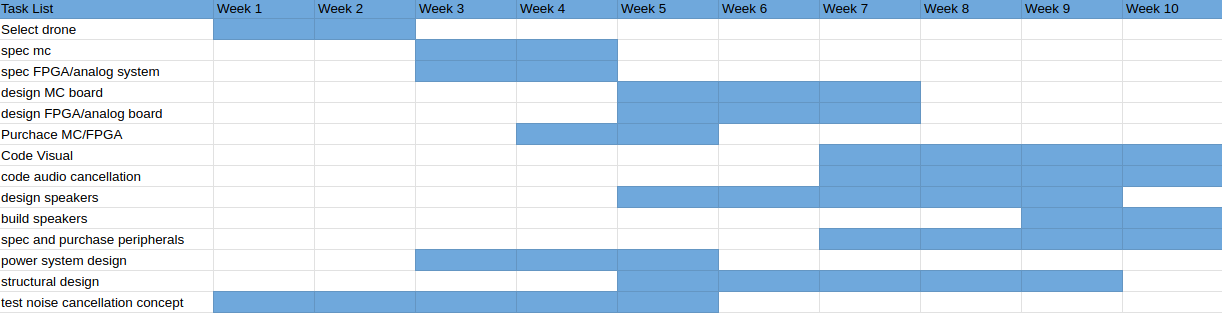
\includegraphics[width=15cm]{timeline.png}
%\caption{Project Gantt Chart}
%\label{fig:timeline}
%\end{figure}

\begin{figure}[H]
    \centering
    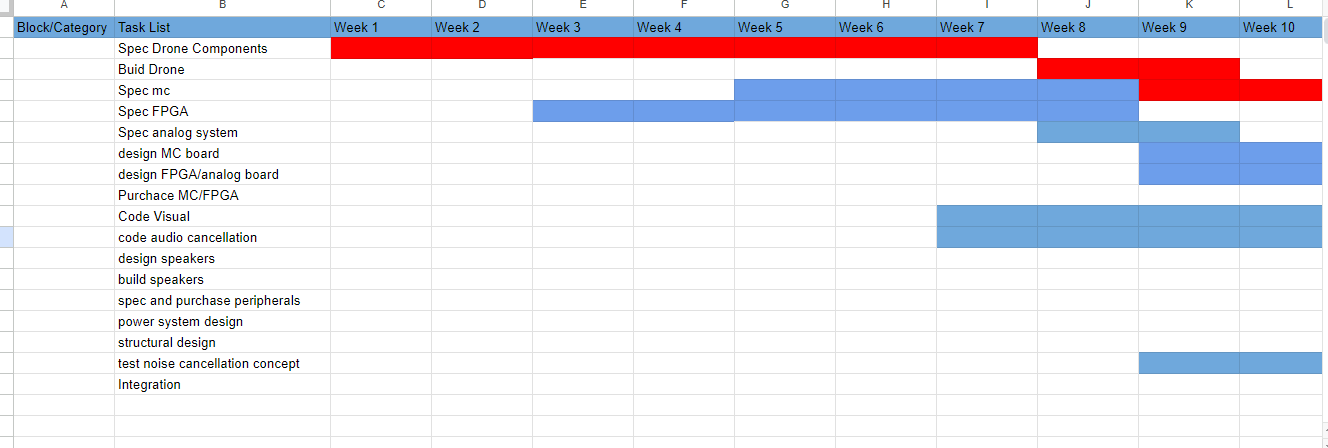
\includegraphics[width=0.5\linewidth]{images/TimelineWk10.png}
    \caption{Gantt Chart Wk1-10}
    \label{fig:TimelineWk1-10}
\end{figure}

\begin{figure}[H]
    \centering
    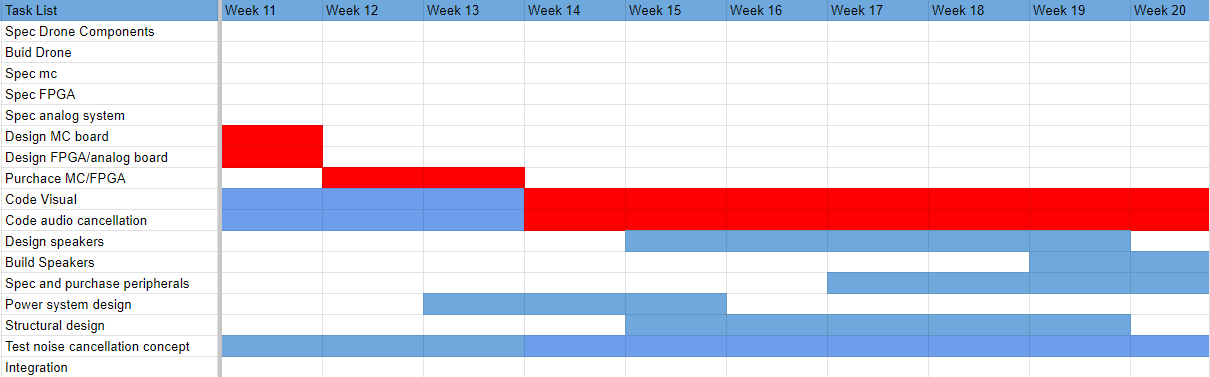
\includegraphics[width=0.5\linewidth]{images/TimelineWk20.png}
    \caption{Gantt Chart Wk11-20}
    \label{fig:TimelineWk11-20}
\end{figure}

\begin{figure}[H]
    \centering
    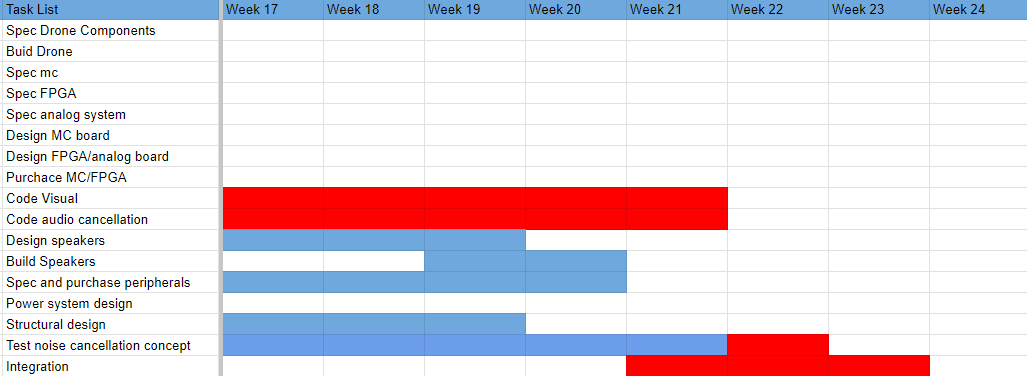
\includegraphics[width=0.5\linewidth]{images/TimelineProjClose.png}
    \caption{Gantt Chart Wk21-Conclusion}
    \label{fig:TimelineWk21-Concluion}
\end{figure}
\subsection{Revision Table}
\begin{table}[H]
\centering
\begin{tabular}{|c|c|c|} % don't change justification. if necesary to change, message is too long
  \hline
  \textbf{Date} & \textbf{Name} & \textbf{Description of Change} \\ 
  \hline
  11/21 & Evan & Updated Project Timeline and related figures; Updated project overview to include S2 \\
  
  \hline
  11/11 & Evan & Updated Task list to reflect progress\\
  \hline
  10/20 & All & Initial document creation  \\
  \hline
  10/15 & Silas & Created \LaTeX\ project and set up GitHub integration. \\ 
  \hline
\end{tabular}
\end{table}
\end{refsection}

\begin{refsection}
\section{Impacts and Risks}
\setcounter{table}{0}  %!!!!!!!!!!!!! if there's a abetter way to do this then do it -Evan
% What is this for? -Silas
\subsection{Design Impact Assessment}
Impact assessment underway. Please reach out to team members as detailed in section 1.2 if additional information is needed. 
\subsection{Risks}
\subsubsection{Risk assessment}
There are several risks inherent in every project, particularly those that adhere to a strict schedule. Within our project, we identified 4 primary risk categories: time-related, budgetary, feasibility, and marketing.  \par
Time-related risks are scenarios that may impact the group's ability to stick to the timeline outlined in section 1.4. Budget-related risks are risks that don't necessarily critically diminish the end result but will cost money and thus reduce the end-product value and the group's ability to continue product development. Feasibility risks are those which critically undermine the technology that is under development. These are things that may make the project impossible. Marketing risks are those that reduce the product's marketability in the end stages. \par
The risks that the group has identified for the LNVD project are summarized below in Table 1. 
\begin{table}[H]
 \caption{Risk Table} 
  \centering
\resizebox{\textwidth}{!}{\begin{tabular}{|c|c|c|c|c|c|}
 
  \hline
  \textbf{Risk ID} & \textbf{Risk Description} & \textbf{Risk Category} & \textbf{Risk Probability} & \textbf{Risk Impact} & \textbf{Action Plan} \\ 
  \hline
  R1 & Vendor Delay & Timeline & H & M & Provide timeline padding \\
  \hline
  R2 & Member sickness & Timeline & H & L & Request help when its needed \\
  \hline
  R3 & Insufficient drone payload & Budget/Timeline & L & H & Full team checkoff on drone purchase \\
  \hline
  R4 & Break components & Budget/Timeline & M & M & Purchase extras when possible \\
  \hline 
  R5 & Majority constructive interference & Feasibility & L & H & Calculate speaker/mic positioning \\
  \hline
  R6 & Insufficient battery & Marketing & H & L & Emphasize low power functionality \\
  \hline  
  R7 & Exceeding thermal characteristics of wires & Feasibility & L & M & Replace provided wires with higher gauge \\
  \hline
\end{tabular}}
\end{table}
\subsubsection{Risk Specific Notes}
R6 - Market research motivated by "Iterate" recommended investigating the specific needs of our target market. One of the primary risks we identified within this niche is the expected duration of most photographed events. For example, standard weddings are approximately 6 hours long \cite{WeddingStats}. While the technology the group is developing is intended as a prototype for which better drone technology can be applied at a later date, our current estimation of our battery will be 30 seconds. Therefore, extrapolating the increased price of 1000 times the battery capacity may exclude members of our target market. It is therefore quite necessary to reduce power as much as possible to support the future customer's requirements. 
\subsection{References}
\printbibliography[heading=none]


\subsection{Revision Table}
\begin{table}[H]
\centering
\begin{tabular}{|c|c|c|} % don't change justification. if necesary to change, message is too long
  \hline
  \textbf{Date} & \textbf{Name} & \textbf{Description of Change} \\ 
  \hline
   11/21 & Evan & Updated section 2 per administration's recommendations; Added R7 to table 1. \\
  \hline
  11/11 & All & Initial creation of Section 2. \\ 
  \hline
\end{tabular}
\end{table}
\end{refsection}


\begin{refsection}
\section{Top-Level Architecture}
\setcounter{table}{0}
\setcounter{figure}{0}

\subsection{Block Diagram}
\begin{figure}[H]
\centering
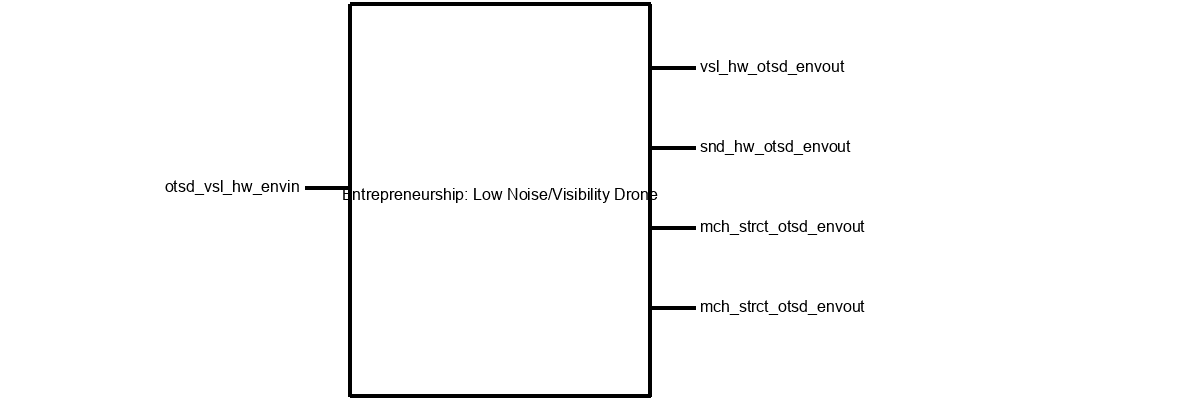
\includegraphics[width=8cm]{images/blackbox.png}
\caption{Black box diagram of the system.}
\label{fig:blackbox}
\end{figure}

\subsection{Block Descriptions}
\subsubsection{Visual HW}

\begin{figure}[H]
    \centering
    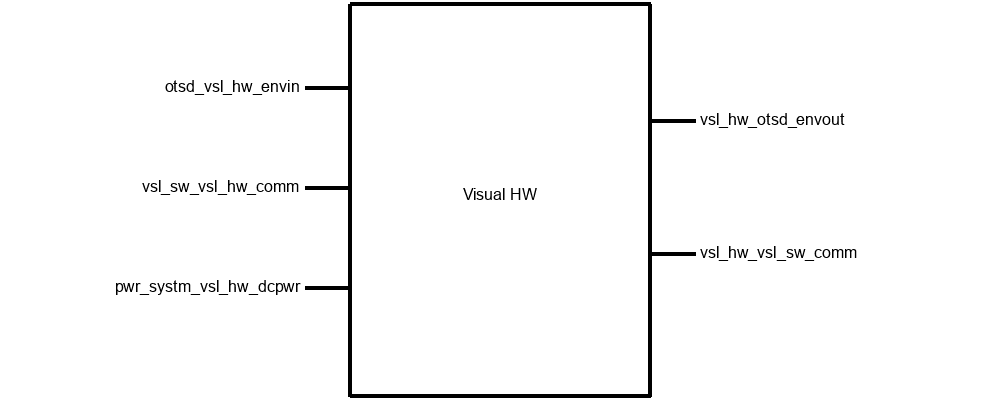
\includegraphics[width=0.5\linewidth]{images/VisualHW_Block_12_1.png}
    \caption{Visual HW Black Box}
    \label{fig:enter-label}
\end{figure}

\par This work block entails the hardware pertaining to the visual camouflage system. This includes the microcontroller’s layout as well as all necessary peripherals such as light display, camera etc. The hardware will function to capture the visual environment, pass it to the visual software block and then generate the appropriate image based on the software commands.

\subsubsection{Visual SW}

\begin{figure}[H]
    \centering
    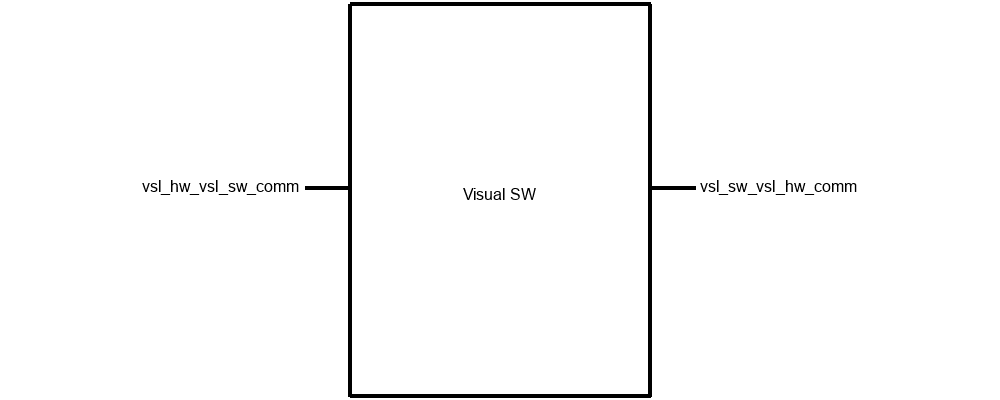
\includegraphics[width=0.5\linewidth]{images/Visual_SW_Block_12_1.png}
    \caption{Visual Software Black Box}
    \label{fig:enter-label}
\end{figure}

\par This work block entails the microcontroller’s software which controls the drone’s visual camouflage. This includes all software levels necessary to interface with the hardware peripherals. It will receive as an input the environmental lighting from the hardware and produce as an output the appropriate lighting for the hardware to generate.


\subsubsection{Sound HDL}
\begin{figure}[H]
    \centering
    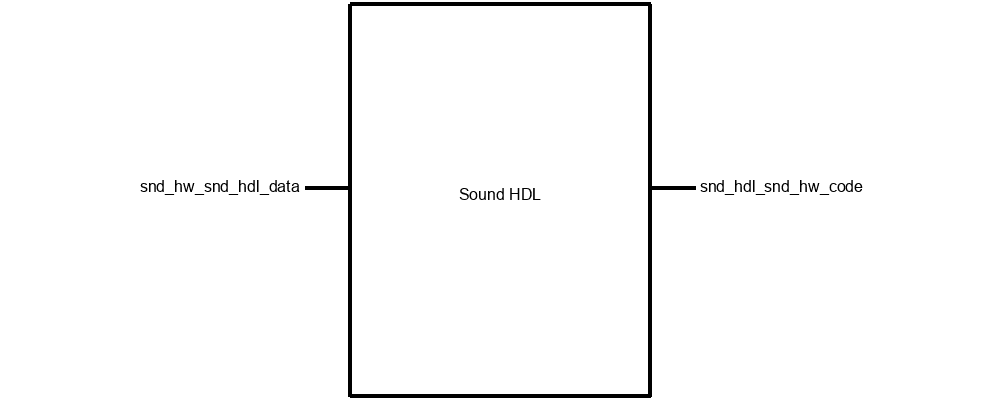
\includegraphics[width=0.5\linewidth]{images/Sound_HDL_12_1.png}
    \caption{Sound HDL Black Box}
    \label{fig:enter-label}
\end{figure}
\par This work block entails the software pertaining to the FPGA’s control of the sound system. This includes all software levels necessary to interface with the hardware peripherals. The HDL will take as an input the acoustic noise generated by the mechanical structure. Subsequently the HDL will, with maximum speed, produce the inverted acoustics subtracting the buffered previous outputs \cite{noiseCancelArticle}. Similar software has been implemented in cars to reduce broad-band noise from the road \cite{carCancellation}. 

\subsubsection{Sound HW}

\begin{figure}[H]
    \centering
    \includegraphics[width=0.5\linewidth]{images/Sound_HW_12_1.png}
    \caption{Sound HW Black Box}
    \label{fig:enter-label}
\end{figure}


\par This work block entails the hardware pertaining to the sound canceling system. This includes the FPGA’s layout as well as all necessary peripherals. It will take as an input the environmental noise generated by the mechanical structure, and pass it to the HDL block. Subsequently it will receive as an input the digital audio signal produced by the HDL and propagate this noise within the environment.
\subsubsection{Mech Struct}
\begin{figure}[H]
    \centering
    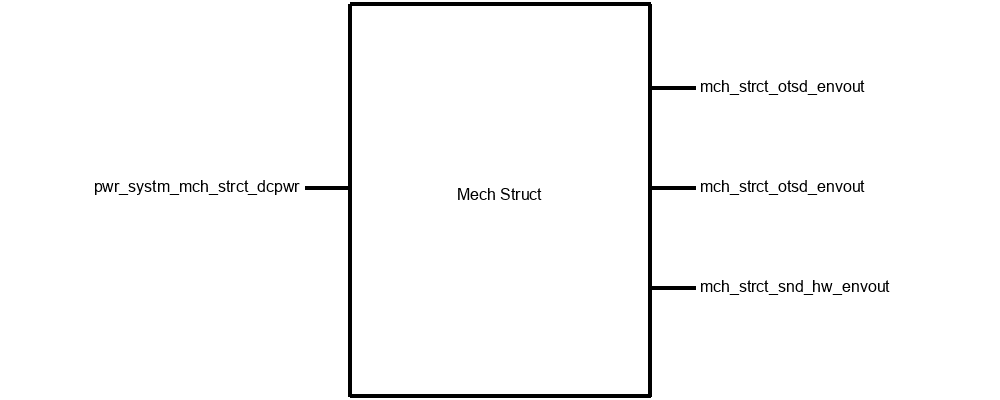
\includegraphics[width=0.5\linewidth]{images/mech_struct_12_1.png}
    \caption{Mech Struct Black Box}
    \label{fig:enter-label}
\end{figure}
\par The mechanical structure will encompass the mechanical connection between drone, camouflage, and noise-cancellation subsystems. The connections will maximize aerodynamic potential and acoustic function. The mechanical structure will also include the drone subsystem which will contribute flight capability.
\subsubsection{Power System}
\begin{figure}[H]
    \centering
    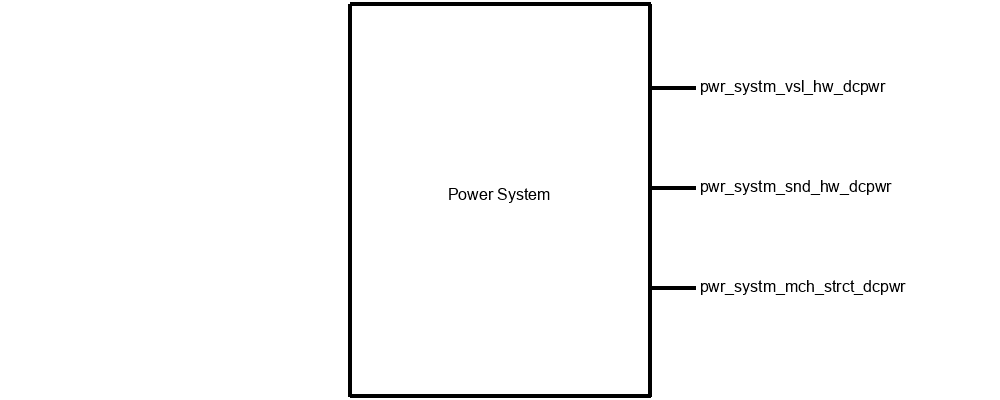
\includegraphics[width=0.5\linewidth]{images/power_system_12_1.png}
    \caption{Power System Black Box}
    \label{fig:enter-label}
\end{figure}
\par This block will produce the power electronic designs and implementations used for providing the power requirements, i.e. current and voltage, required by the other electrical systems. Based on the subsystem requirement, the power system will generate the required values. This includes all voltage and current supplies.

\subsection{Interface definition}
\begin{figure}[H]
    \centering
    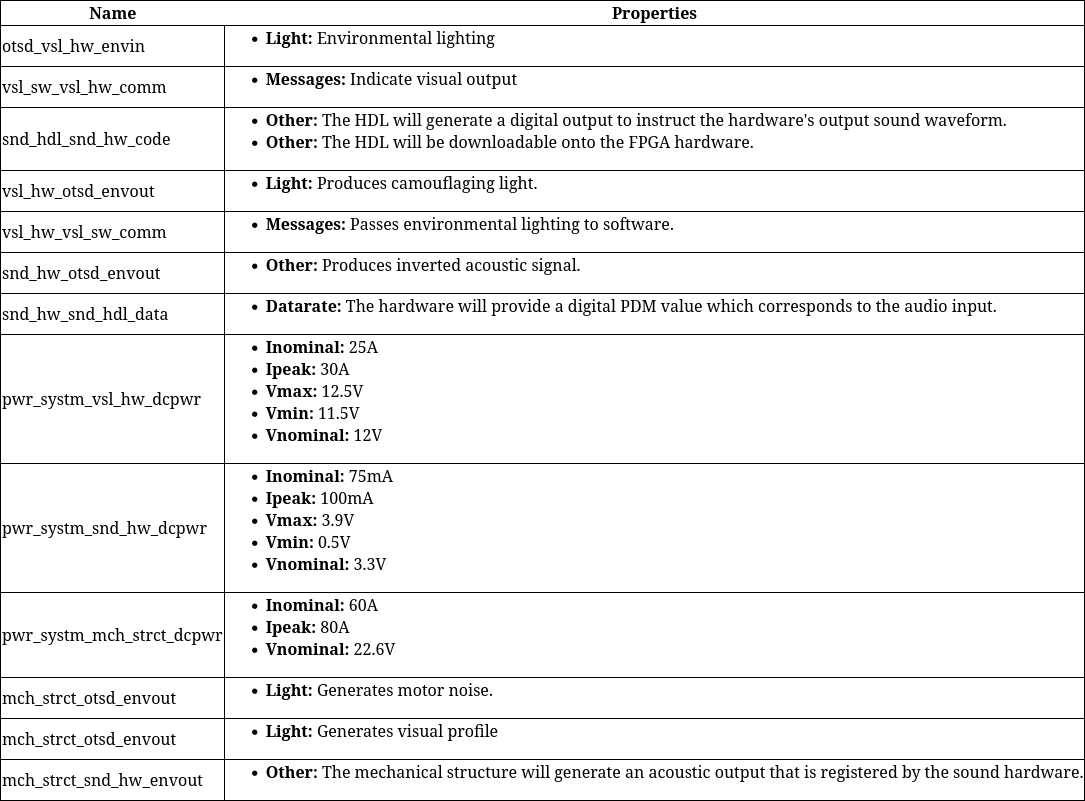
\includegraphics[width=0.5\linewidth]{images/interfaceshit.png}
    \caption{Interface definition table}
    \label{fig:interface}
\end{figure}
\subsection{References}
\printbibliography[heading=none]

\subsection{Revision Table}
\begin{table}[H]
\centering
\begin{tabular}{|c|c|c|} % don't change justification. if necesary to change, message is too long
  \hline
  \textbf{Date} & \textbf{Name} & \textbf{Description of Change} \\ 
  \hline
  12/1 & All & Initial creation of Section 3. \\ 
  \hline
\end{tabular}
\end{table}


\end{refsection}

\begin{refsection}
\section{Block Validations}
\setcounter{table}{0}

\end{refsection}


\begin{refsection}

\section{System Verification Evidence}
\subsection{Universal Constraints}
\par The system will follow the universal constraints that are enumerated in the subsequent sections. 
\subsubsection{The system may not include a breadboard.}
\par The final system shall not contain any breadboards, protoboards, or "dead bug" prototype boards. All components will be placed on a PCB or on their own with connectors connecting them to a PCB. 
\subsubsection{The final system must contain a student designed PCB.}
\par The final system will include at least one custom PCB controlling power, visual, and audio. The PCB or PCBs will be designed using KiCad and sent to Osh Park for fabrication. 
\subsubsection{All connections to PCBs must use connectors.}
\par All the external modules such as the battery, LCDs, speakers, microphone, and camera will be connected to our PCB using connectors. 
\subsubsection{All power supplies in the system must be at least 65\% efficient.}
\par Any power electronics in the system will be chosen such that the overall efficiency of the system is at least 65\%. 
\subsubsection{The system may be no more than 50\% built from purchased `modules.'}
\par None of our blocks will be pre-built, meaning that 0\% of our system will be built from purchased `modules.'
\subsection{Requirements}

\newcommand{\Requirement}[6]{
    \subsubsection{#1}
    %subsubsub DNE so use this.  I set the section counter to allow this; if we need another number we can use subparagraph -Evan
    %Customer Requirement
    \paragraph{Customer Requirement}
    \paragraph*{
    \textnormal{#2}
    }
    
    %Engineering Requirement
    \paragraph{Engineering Requirement}
    \paragraph*{
    \textnormal{#3}
    }
    
    %Tesing Method
    \paragraph{Testing Method}

    \textnormal{#4}
    
    
    %Verification Process
    \paragraph{Verification Process}
    \paragraph*{
    \textnormal{#5}
    }

    %Testing Evidence
    \paragraph{Testing Evidence}
    \paragraph*{
    \textnormal{#6}
    }
}

\Requirement{Active Camouflage Controllability}
{The drone is controllable and well documented.}
{The visual camouflage and noise-canceling subsystems will operate independently once the system's power is engaged.}
{
    \begin{enumerate}
        \item Ensure the drone is off.
        \item Turn the drone on.
        \item Verify that the visual camouflage and noise-canceling subsystems are powered and operating normally
    \end{enumerate}
}
{Demonstration.}
{}

\Requirement{Battery Life}
{The drone can fly independently.}
{The system will last for at least 25 seconds while hovering above the ground by at least 1 inch.}
{
    \begin{enumerate}
        \item Ensure the drone is off.
        \item Turn the drone on.
        \item Start a timer and fly the drone to 6 ft; make the drone hover.
        \item Wait for at least 25 seconds
        \item Land the drone, and stop the timer.
        \item Visually verify that the drone was flying and both visual camouflage and noise-canceling subsystems were active for at least 25 seconds.
    \end{enumerate}
}
{Testing.}
{}

\Requirement{CAD Model}
{The drone is controllable and documented.}
{The project will produce a CAD model that shows how the camouflage and noise-canceling subsystems are mechanically mounted to the drone subsystem with a fully defined model that describes geometric matings between subsystems to within 0.5 inches.}
{
    \begin{enumerate}
        \item Open the CAD Model
        \item Check that each of the subsystem models are described by mates within 0.5 inches.
    \end{enumerate}
}
{Inspection.}
{}

\Requirement{Documentation}
{The drone is controllable and documented.}
{The project will produce a standard-operating-procedure (SOP) document that explains how to start the drone, basic drone controls, and how to disable/enable the camouflage and noise-canceling subsystems such that 9 out of 10 users can successfully initiate flight with active camouflage and noise-cancellation.}
{
    \begin{enumerate}
        \item For each of the 10 participants, give the participant the SOP document; tell them to use the SOP to do the following:
        \begin{enumerate}
            \item Ensure the drone is off.
            \item Turn on the drone.
            \item Turn on the camouflage and noise-canceling subsystems.
            \item Fly to 6 feet.
            \item Hover the drone for a few seconds.
            \item Land the drone.
            \item Turn off the drone.
            \item Turn off the camouflage and noise-canceling subsystems.
        \end{enumerate}
        \item Verify that 9 out 10 participants were able to successfully complete the verbal instructions.
    \end{enumerate}
}
{Testing.}
{}

\Requirement{Flyabillity}
{The drone can fly independently.}
{The system will leave the ground and ascend to a height of at least 5 yards without any external connections.}
{
    \begin{enumerate}
        \item Ensure the drone is off
        \item Turn on the drone
        \item Turn on the camouflage and noise-canceling subsystems.
        \item Fly the drone to a height of at least 5 yards.
        \item Verify that the drone has no external connections
        \item Land the drone.
    \end{enumerate}
}
{Testing.}
{}

\Requirement{Form Factor}
{The system fits small indoor spaces.}
{The system will fit within 18x18x18 inches cubed.}
{   
    \begin{enumerate}
        \item Place the drone on a flat surface.
        \item Rotate an 18 inch measuring tool starting from its endpoint such that the drone's length, width, and height can be compared.
        \item For each dimension verify that the drone's profile is less than the 18 inch length of the measuring tool
    \end{enumerate}}
{Testing.}
{}

\Requirement{Noise Reduction}
{The drone is quiet}
{The system noise is reduced by -4dB at a point on the ground exactly 6 feet below the drone when the noise-cancelling subsystem is engaged.}
{
    \begin{enumerate}
        \item Ensure the room is quiet.
        \item Ensure the drone is off.
        \item Turn on the drone.
        \item Ensure the camouflage and noise-canceling subsystems are off.
        \item Fly the drone directly above the recording microphone at a height of 6 feet.
        \item Make the drone hover.
        \item Record the noise emitted from the drone for 10 seconds.
        \item Land the drone.
        \item Turn off the camouflage and noise-canceling subsystems.
         \item Fly the drone directly above the recording microphone at a height of 6 feet.
        \item Make the drone hover.
        \item Record the noise emitted from the drone for 10 seconds.
        \item Land the drone.
        \item Compute the proportional average power of each recording. (Note that the actual power is
              dependent on the sensitivity of the microphone used; however, so long as the same microphone is used for both recordings, an accurate comparison can be made without knowing the actual power.)
        \item Verify that the recording in which the noise-canceling subsystem is engaged has an average power
              4 dB less than the recording where the subsystem was off.
    \end{enumerate}
}
{Testing}
{}

\Requirement{Visual Profile Reduction}
{The drone is difficult to see.}
{After taking a picture of the drone with and without the camouflage in the same place, 9 out of 10 people will say the drone is harder to see in the picture where camouflage was enabled versus that in which it was not enable.}
{
    \begin{enumerate}
        \item Ensure the drone is off.
        \item Turn on the drone.
        \item Ensure the camouflage and noise-canceling subsystems are off.
        \item Fly the drone directly above the camera at a height of 6 feet.
        \item Make the drone hover.
        \item Record a video of the drone for 10 seconds.
        \item Land the drone.
        \item Turn off the camouflage and noise-canceling subsystems.
        \item Fly the drone directly above the camera at a height of 6 feet.
        \item Make the drone hover.
        \item Record a video of the drone for 10 seconds.
        \item Land the drone.
        \item For each of the 10 participants:
        \begin{enumerate}
            \item Show them one of the videos (selected at random).
            \item Show them the other video.
            \item Ask whether the drone was easier to see, harder to see, or the same in the first video versus the second video.
            \item Write down their response.
        \end{enumerate}
        \item Verify that 9 out of 10 participants reported the drone was harder to see when the camouflage subsystem was active versus when it was disabled.
    \end{enumerate}
}
{Testing}
{}

\subsection{Revision Table}
\begin{table}[H]
\centering
\begin{tabular}{|c|c|c|} % don't change justification. if necesary to chhange, message is too long
  \hline
  \textbf{Date} & \textbf{Name} & \textbf{Description of Change} \\ 
  \hline
  12/1 & All & Initial creation of Section 5. \\ 
  \hline
\end{tabular}
\end{table}
\end{refsection}

\begin{refsection}
\section{Project Closing}
\setcounter{table}{0}

\end{refsection}

\end{document}